\documentclass[UTF8]{ctexart}
\usepackage{graphicx}
\usepackage{listings}

\title{实验五报告}
\author{唐灵\\519030910052\\F1903002}
\date{\today}
\begin{document}
    \maketitle
    \begin{abstract}
        这是电工导c课程的第四次实验
    \end{abstract}
    \section{实验概览}
        本次实验是对于爬虫与文本检索的一个综合简单应用,重点在于应用lucene建立索引实现简单的组合搜索,以及图像搜索。
    \section{实验环境}
    本次实验并未在课程方统一给定的“ee208”$Docker$容器中运行并实现。

    本次实验由于环境问题,没有办法在个人电脑上运行indexfile文件,上次实验选择在别的同学电脑上完成程序的编写,并迟交了一段时间,而这次实验,可能由于学业繁忙,没有找到合适的同学。

    所以最终选择在无参考方式下阅读周毓519030910049同学的代码,并独立完成报告,对于文本检索的实际应用进行学习。
    \section{练习解决思路}
        \subsection{练习一的解决思路}
            针对爬虫模块,解决思路与我个人的实验四不同,采用了在爬取的过程中,固定的将其特定属性写入html文档中,也就是事先进行信息处理和分析,
            将文本信息,开头,url,文件名等等信息按照一定的顺序存储在开头,在建立索引的过程中可以直接使用。

            针对建立索引模块,为了能够事先组合搜索,我们需要将url,title等等信息预先进行分词,方便之后的组合查询。
            \begin{figure}[ht]
                \centering
                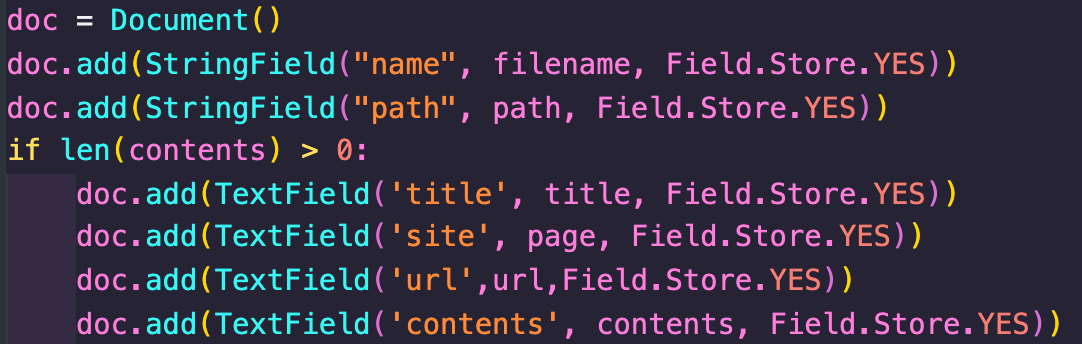
\includegraphics[scale=0.5]{img/str.png}
                \caption{加入字段}
            \end{figure} 

            针对与搜索模块,我们对于输入的字段进行自定义的处理,构造字典,使得其能够满足布尔查询的方法。
            \begin{figure}[ht]
                \centering
                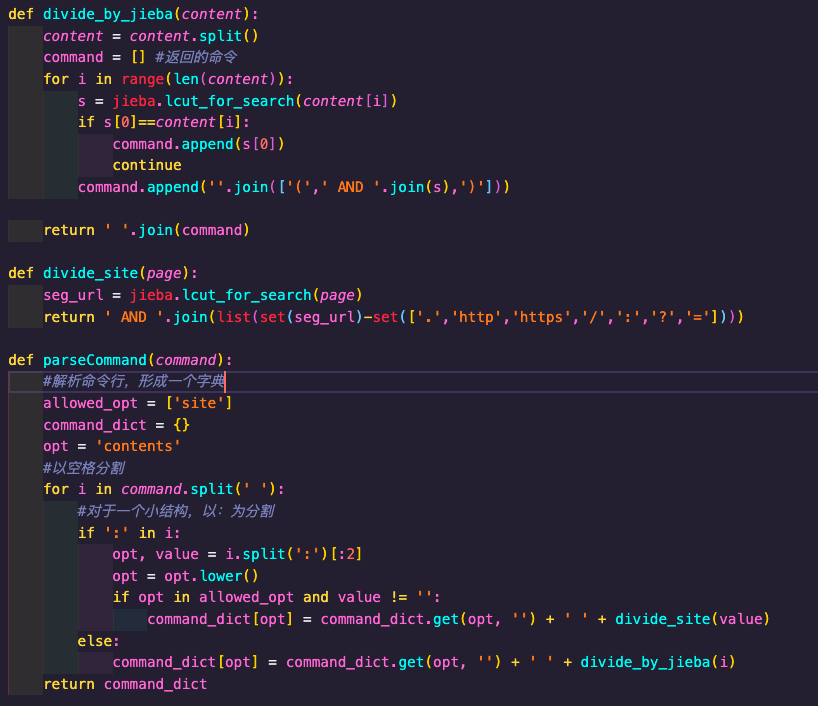
\includegraphics[scale=0.2]{img/deal.png}
                \caption{对于搜索字段进行处理}
            \end{figure}

        \subsection{练习二的解决思路}
            对于练习二的解决思路和一般的检索思路相同。

            关键点在于爬取的时候,从图片的周围抽取图片信息来进行字段的搜索存储,用于字段的搜索。

    \section{代码运行结果}
        \subsection{练习一的运行结果}
        \begin{figure}[ht]
            \centering
            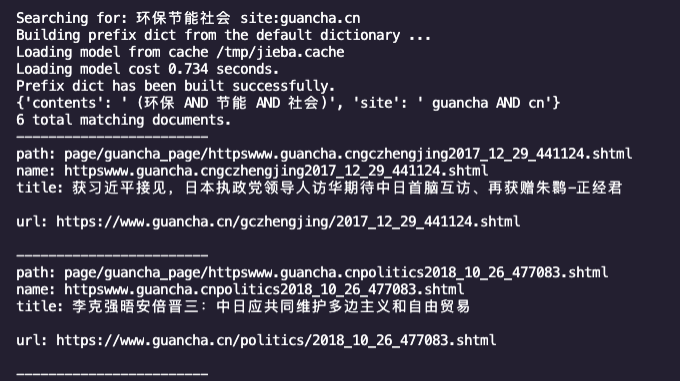
\includegraphics[scale=0.3]{img/search_sina.png}
            \caption{对于域名为sina的搜索结果}
        \end{figure} 
        \begin{figure}[ht]
            \centering
            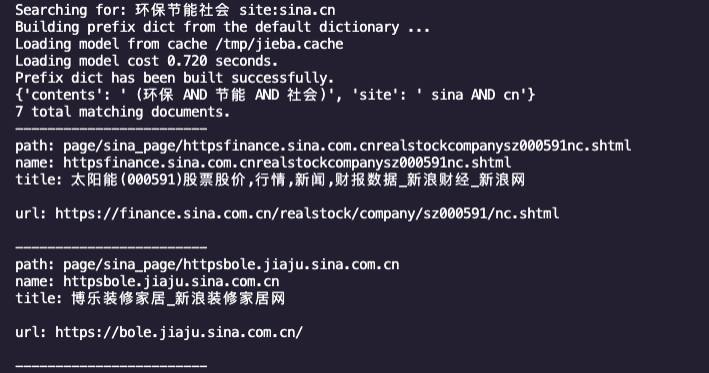
\includegraphics[scale=0.3]{img/search_guancha.png}
            \caption{对于域名为guancha的搜索结果}
        \end{figure} 
        \subsection{练习二的运行结果}
        \begin{figure}[ht]
            \centering
            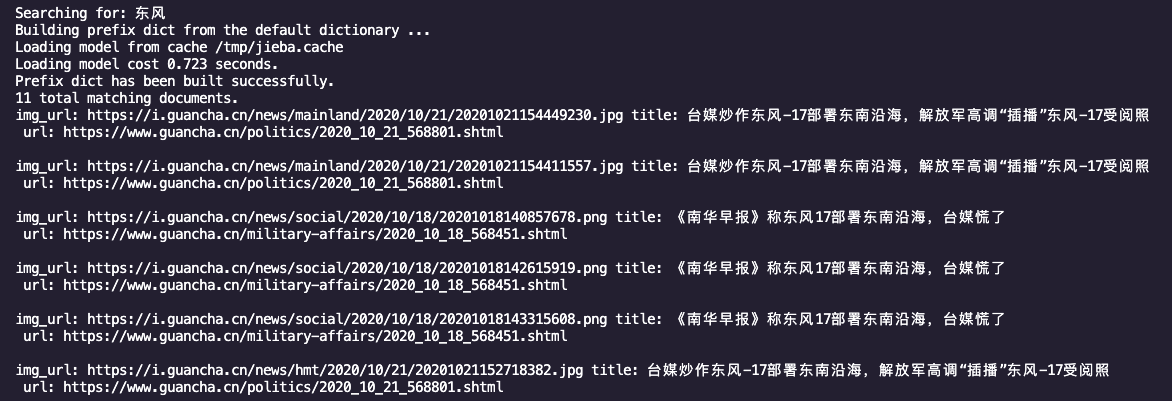
\includegraphics[scale=0.3]{img/search_ph.png}
            \caption{搜索图片结果}
        \end{figure} 

\end{document}